% !TEX root = main.tex
\chapter{Experimental techniques}
\label{chap:tools}

\linespread{1.08}\selectfont
In this chapter several experimental techniques used in the analysis are introduced.
First, three statistical tools are described:
a multivariate classifier called \ac{BDT} is described in \cref{sec:BDT} based on Ref.\cite{Bohm:389738}.
In the analysis, \ac{BDT}s are used in the selection of \BdToDpi candidates and when determining the production flavour of the \Bz mesons.
The maximum-likelihood method which is used to fit the invariant \Bz mass and to estimate the \CP asymmetries is detailed in \cref{sec:MLFit}~\cite{Bohm:389738}.
The last statistical tool, the \emph{sPlot} technique~\cite{Pivk:2004ty}, is described in \cref{sec:splot}, which is used to statistically separate signal from background candidates.
Finally, the flavour tagging is introduced in \cref{sec:flavourtagging}, which provides algorithms to infer the initial flavour of \Bz and \Bs mesons at \lhcb.

\section{Boosted decision trees}
\label{sec:BDT}

Decision trees are multivariate classifiers, \ie they analyse multiple randomly distributed variables simultaneously in contrast to simple univariate analyses that examine each variable individually.
A decision tree classifies a data set of different types of events by applying hierarchically ordered logical rules to different properties of these events.
The tree always consists of a root node and an arbitrary number of sub nodes, as well as at least two leaves.
For binary decision trees, as used in the scope of this thesis, the rule applied at each node has only two possible outcomes.
Figure \ref{fig:BDTexample} shows a decision tree with a depth of two, \ie two consecutive binary decisions are made before the events are assigned to the classes $A$ and $B$, depending on their final leave.
\begin{figure}[tbp]
    \centering
    \includestandalone{06tools/figs/BDT}
    \caption{Binary decision tree with a depth of two, dividing events into the classes $A$ and $B$ based on the variables $v_i$.}
    \label{fig:BDTexample}
\end{figure}
In principle, each decision tree starts applying a rule to the variable with the best separation power (here $v_1$) in the root node.
Subsequently, further rules are applied in the lower sub nodes until certain limits are reached, \eg a minimum number of events in each leave.

Before applying a decision tree to a data sample, first it needs to be trained with data samples labelled according to their class.
Furthermore, an estimate of the separating power of the different variables is needed.
An easy way for example is to maximise the difference $\Delta N=N_r-N_w$ between right ($N_r$) and wrong ($N_w$) assignments in a node.
However, the cut point of the binary rule remains random to some extent, since the value $\Delta N$ only changes when the cut-point is shifted by so much that it hits the nearest variable value.
A slightly more complicated, but very popular measure is the following:
the purity $P$ of events from class $A$
\begin{equation}
P_A=\frac{N_A}{N_A+N_B}\,,
\end{equation}
where $N_i$ are the number of events from class $A$ and $B$, becomes $0$ or $1$ if the classification is perfect.
Therefore, minimising the Gini Index~\cite{Bohm:389738}
\begin{equation}
G=P_A\left(1-P_A\right)+P_B\left(1-P_B\right)
\end{equation}
provides presumably the variable with the largest separation power.
As the selection of variables depend on the chosen variables and applied cuts in higher nodes of the decision tree, correlations are automatically taken into account.

The overall classification performance can be improved by not only using one moderately effective classifier but instead calculating the weighted average of many different decision trees.
In order to do so, many decision trees are grown.
Each time a new tree is built, events, which were assigned to the wrong class by the previous tree, are weighted (boosted) in order to reduce the probability that they are wrongly classified again.
Such a combination of decision trees is denoted as boosted decision tree (\ac{BDT}).
Well known boosting algorithms are the gradient boosting technique~\cite{gradientBoost} or the adaptive boosting (AdaBoost) method~\cite{AdaBoost}.
Since the latter is used in the selection of \BdToDpi candidates in \cref{chap:selection} and the development of flavour-tagging algorithms in \cref{ch:flavourtagging} it is shortly described here.

Considering a boosted decision tree consisting of $T$ trees, where the trees are distinguished by the subscript $t$.
The first decision tree is trained with $N$ events equally weighted providing a hypothesis $h_1(x^i)$ being \num{+1} (\num{-1}) for signal (background) for the $i$-th event.
This hypothesis is compared with the label $y_i$ and the total error rate is calculated as
\begin{equation}
\varepsilon_1=\sum_{i=1}^{N}p^i_1\left|h_1(x^i)-y^i\right|\,,
\end{equation}
where $p_1^i=\nicefrac{w_1^i}{\sum_{i}w_1^i}$ is the normalised weight for each event.
This can be generalised by replacing the subscript $1$ with $t$.
Using this error rate the weights for the next tree are computed using the boost weight
\begin{equation}
\alpha^i=\left(\frac{\varepsilon_t}{1-\varepsilon_t}\right)^{\beta\left(1-\left|h_t(x^i)-y^i\right|\right)}
\end{equation}
as $w_{t+1}^i=\alpha w_t^i$, where $\beta$ is the boosting factor,  which, in simple terms, modifies the learning rate during the training.
The final BDT output is then given by
\begin{equation}
h_f(x^i)=\frac{1}{T}\sum_{i=1}^{T}\ln\left(\alpha^i\right)\times h_t(x^i)\,,
\end{equation}
which is distributed between \num{-1} and \num{+1}, implying that an event is more likely signal (background) when the value is close to \num{+1} (\num{-1}).

When training a \ac{BDT}, some caveats must be taken into account.
On the one hand, the labelled data samples used in the training are usually only proxies for the \emph{real} data.
For example, differences between simulated events and \emph{real} data can lead to a bad performance of the \ac{BDT}.
Furthermore, the \ac{BDT} can learn to distinguish the training data samples by statistical fluctuations.
This phenomenon, denoted as over-fitting or overtraining, can be avoided by splitting the labelled training data sample before developing the \ac{BDT}.
The first half is then used as training data set and following the \ac{BDT} is applied to the second data set denoted as test sample.
If the \ac{BDT} output distributions on both data sets are the same, it can be assumed that there is no overtraining.

To train \ac{BDT}s, various implementations exist.
In the course of this thesis always the implementation from TMVA~\cite{Hocker:2007ht} is used.


\section{The maximum-likelihood method}
\label{sec:MLFit}

The maximum-likelihood method is a common tool for parameter estimation from a data sample.
In simple terms, the parameter values are selected as an estimate according to which the shape of the observed data appears most probable.
This estimation is possible in either one or multiple dimensions.
Assuming $n$ measurements of a set of observables $\vec{x}$ the maximum-likelihood function is given as
\begin{equation}
\mathcal{L}(\vec{a})=\mathcal{P}(\vec{x}_1|\vec{a})\times\mathcal{P}(\vec{x}_2|\vec{a})\times...\times\mathcal{P}(\vec{x}_n|\vec{a})=\prod_{i=1}^{n}\mathcal{P}(\vec{x}_i|\vec{a})\,,\label{eq:mlfunc}
\end{equation}
where $\mathcal{P}(\vec{x}_i|\vec{a})$ are the properly normalised probability densitiy function (PDF) with a set of parameters $\vec{a}$ to estimate.
The function $\mathcal{L}(\vec{a})$ gives the probability of obtaining the measured values for a set of parameters $\vec{a}$ in a sample $\vec{x}_i$.
However, even if the maximum-likelihood function becomes maximal for the maximum probability of obtaining the data set $\vec{x}_i$, it is not a probability density in the parameters $\vec{a}$.
Extending the function in \cref{eq:mlfunc} with a Poisson term
\begin{equation}
\mathcal{L}(\vec{a})=\frac{e^{-n}n^N}{N!}\prod_{i=1}^{n}\mathcal{P}(\vec{x}_i|\vec{a})\,,
\end{equation}
where $n$ is the number of expected events, although the sample containts $N$ measurements allows to distinguish different categories of events by summing up several likelihood functions.
Usually, the negative logarithmic likelihood function is minimised because this is numerically more stable and it leads to the same results, since the logarithm is a monotone function.

Besides, it is possible to use an external input to constrain a parameter $\mu$ to be $\mu_0\pm\Delta\mu$ by means of a Gaussian function.
This implies that the likelihood is multiplied by a Gaussian with the mean and width set to $\mu_0$ and $\Delta\mu$, respectively.
In this analysis, the maximum-likelihood fits were implemented using the \root framework~\cite{Antcheva:2009zz}, which makes use of the Minuit package~\cite{James:1975dr} for the minimisation of the likelihood function.


\section{The sPlot technique}
\label{sec:splot}

The \emph{sPlot} technique~\cite{Pivk:2004ty} uses a maximum-likelihood fit to calculate the so-called \emph{sWeights} by performing a \emph{sPlot} fit to one or multiple discriminating observables.
Considering a data sample, containing a mixture of $N_c$ different categories of events, the \emph{sWeights} are per-event weights ${}_sw$, which allow to reconstruct the distributions of variables separately for each category present in the initial sample.
However, one important assumption is that the \emph{sWeights} are applied to observables, which are independent of the discriminating observables.
To perform a \emph{sPlot} fit the PDFs for all categories of events are needed, so that the \emph{sWeights} can be calculated as
\begin{equation}
{}_sw=\frac{\sum_{j=1}^{N_c}V_{nj}\,f_j(\vec{y}_e)}{\sum_{k=1}^{N_c}N_k\,f_k(\vec{y}_e)}\,,
\end{equation}
where the sums iterate over all categories of events.
Moreover, the functions $f_i$ are the corresponding PDFs of the discriminating set of observables $\vec{y}$ for an event $e$, $N_k$ is the yield in the corresponding category and $V$ the covariance matrix of the yields.
In practice, a first fit to the observables $\vec{y}$ is performed to determine the parameters of the PDFs $f_i(\vec{y})$, before all parameters except for the yields are fixed and the \emph{sWeights} are calculated in a second fit.
The normalisation of the \emph{sWeights} is such that the sum over the weights for one category provides the number of events $N$ of this category in the sample.
The statistical uncertainty on this number of events is defined for each bin $\delta x$ by
\begin{equation}
\sigma_N=\sqrt{\sum_{e\subset\delta x}({}_sw)^2}\,.
\end{equation}

In the scope of this analysis, signal and background candidates for the signal decay \mbox{\BdToDpi} and for the flavour tagging control modes $\Bz\!\to\jpsi\Kstarz$ and $\Bu\!\to\Dz\pip$ are separated using this technique by performing fits to the invariant mass distributions (more details in \cref{ch:massfit} and \cref{ch:flavourtagging}).
The choice of the invariant mass as discriminating observable has two advantages:
on the one hand, it is independent of the decay-time, for which the distribution of signal candidates is needed to \eg extract the \CP asymmetries.
On the other hand, the distributions of the different contributions in the distribution are well known and allow a reliable parametrisation.

\section{Flavour tagging}
\label{sec:flavourtagging}

To measure interference \CP-violation the production flavour of $B$-mesons under study must be known.
At \lhcb this is inferred using the so-called flavour tagging.
A decision (tag) $d$ whether a \B candidate was initially produced as a \Bz-meson or a \Bzb-meson and a probability-estimate (mistag) $\eta$ of being wrong with this decision is provided by the flavour tagging algorithms (taggers).
They can be divided into two classes: opposite side (OS) and same side (SS) algorithms.
In the following, a general description of the different algorithms available at \lhcb, their performance characteristics and their calibration is given

\subsection{Tagging algorithms}
\label{sec:taggingalgorithms}

At \lhcb several tagging algorithms exist to infer the initial $B$ flavour of which some differ for \Bz and \Bs mesons.
In \cref{fig:taggingalgorithms} a schematic representation of the tagging algorithms for \Bz mesons is shown.
\begin{figure}[tbp]
    \centering
    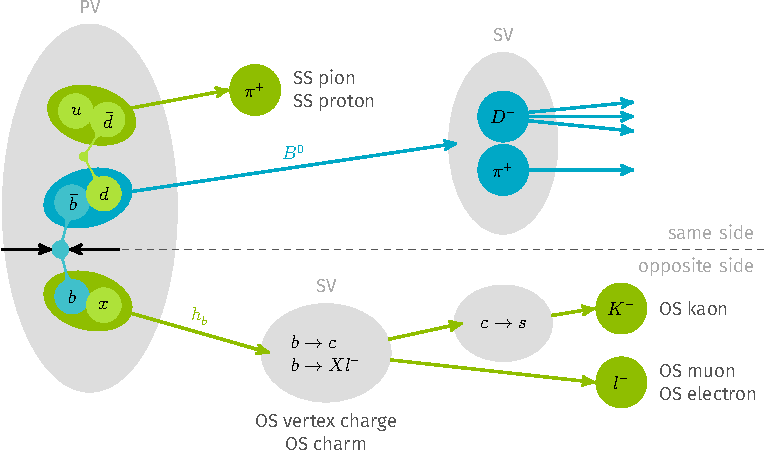
\includegraphics[width=0.8\textwidth]{09FlavourTagging/figs/FTscheme.pdf}
    \caption{Schematic overview of all available \Bz tagging algorithms.}
    \label{fig:taggingalgorithms}
\end{figure}
They can be separated into so-called opposite side (OS) and same side (SS) algorithms.

The OS algorithms exploit the production and decay of the second \bquark-quark which is produced in the proton-proton collision.
By partially reconstructing single decay products as electrons, muons, kaons and \D-mesons associated with the decay of the opposite side \bquark-hadron the initial flavour is inferred.
Furthermore, charged tracks which originate from a secondary vertex, which is displaced from the \ac{PV}, are used to make a decision on the production flavour of the signal $B$-meson.
As the hadronisation and the decay of the OS \bquark-hadron is independent of the signal \B-meson, these algorithms can be used for both \Bz and \Bs mesons. Based on \cite{LHCb-PAPER-2011-027, LHCb-PAPER-2015-027} the OS algorithms are briefly described below:
\begin{itemize}
    \item The OS muon and OS electron tagger use the charge of muons and electrons from semileptonic $\bquark\!\to Xl^-$ decays to take a decision on the initial $B$-flavour.
    The charged leptons are selected using a simple cut-based selection.
    To suppress contributions from $\bquark\!\to\cquark\!\to l^+$ decays, which would give the wrong tag decision, for example the transverse momentum of the muon (electron) is required to be larger than \SI[per-mode=symbol]{1.2}{\GeVc} (\SI[per-mode=symbol]{1.0}{\GeVc}).
    Electrons have additionally to satisfy criteria on electron identification variables such as the ratio $\nicefrac{E}{p}>0.8$.
    Here $E$ denotes the energy deposited in the ECAL and $p$ the electron momentum.
    If more than one muon or electron per event survives the selection, the lepton with the highest transverse momentum is chosen to define the flavour of the signal $B$.
    The mistag is estimated with an artificial neural network, which takes as inputs event properties as the number of \ac{PV}s and tracks in the event, $B$-properties as the transverse momentum and various geometrical and kinematic properties of the tagging lepton.
    \item The OS kaon tagger explores the charge of kaons produced in the decay chain $\bquark\!\to\cquark\!\to\squark$.
    Very similar to the lepton taggers the tagging kaon is selected using rectangular cuts based on kinematic and PID observables.
    In case multiple kaons per event pass this selection, the kaon with the highest transverse momentum is fed into an artificial neural network with similar inputs as for the lepton taggers to calculate the mistag estimate $\eta$.
    \item The OS charm tagger selects \D-mesons produced via $\bquark\!\to\cquark$ decays.
    In case of a charged \D-meson the charge of the meson directly hints at the initial flavour, in case of an uncharged \D-meson the charge of the produced kaon is used to infer the flavour of the signal $B$-meson.
    In contrast to the other single track taggers, a \ac{BDT} is used to select the \D-meson and estimate the mistag.
    As the OS charm is the newest development on the OS it was developed to have a small overlap concerning the used tagging particles with the other taggers.
    \item The OS vertex charge tagger is the only algorithm which does not reconstruct single particles, but uses the weighted charge of a \ac{SV} associated with the opposite side \bquark-hadron instead.
    In order to do this, the track pair with the highest probability of originating from the opposite side \bquark-hadron is used to build a vertex.
    Following, particles which are compatible with coming from this two-track vertex but not from the \ac{PV} are added to it.
    Finally all tracks of the final \ac{SV} are weighted with their transverse momentum, \pt, and used to calculate a charge
    \begin{equation}
    Q_{\text{vtx}}=\frac{\sum_{i}p_{\mathrm T}^k(i)Q_i}{\sum_{i}p_{\mathrm T}^k(i)}\,,
    \end{equation}
    where the parameter $k$ is optimised to maximise the performance of the tagging algorithm.
    Based on this charge the initial flavour of the signal $B$-meson is then determined.
\end{itemize}

The SS algorithms use remnants of the hadronisation of the signal \B-meson to infer the initial flavour.
As the companion quark of the \bquark-quark is different for \Bz and \Bs-mesons, different algorithms must be used to deduce the initial flavour of the signal \B.

In case of a \Bz (\bquarkbar\dquark) a free \dquarkbar-quark is produced which can hadronise to a pion or proton.
Additionally, the production mechanisms, \eg via the strong decay of an excited $B^{**+}\!\to B^{(*)0}\pip$ can be exploited~\cite{Aaij:2016rdg}.
The SS pion and SS proton taggers use the charge of these companion particles to infer a tag decision.
They were developed on \BdToDpi decays assuming $\Sf=\Sfbar=0$, \ie the decay \BdToDpi is \CP-conserving.
Therefore a potential bias of the analysis cannot be excluded when using these algorithms and they are retrained on $\Bz\!\to\jpsi\Kstarz$.
The basic strategy is similar to the one in Ref.~\cite{Aaij:2016rdg}:
First, tagging particles from the same region of phase space as the signal \B are selected using requirements on PID, kinematic and geometrical observables.
Then, these particles are all used to train a \ac{BDT}, which further selects the final tagging particle and estimates the mistag.
This means in case multiple particles per event pass the selection, the SS pion and SS proton taggers do not select the particle with highest transverse momentum but for all particles the \ac{BDT} response is calculated and the tagging candidate with the largest \ac{BDT} response is chosen to infer the initial flavour of the signal \B.

On the other hand the hadronisation of a \Bs (\bquarkbar\squark) leads to a \squarkbar-quark which can hadronise to a kaon~\cite{Aaij:2016psi}.
The SS kaon tagger was developed to identify such kaons and works similar for kaons as the SS pion tagger for pions produced in \Bz events.
Since this analysis covers decays of neutral \Bz mesons and the SS kaon tagger is not used, this algorithm is not discussed any further.

\subsection{Performance characteristics}

The predictions of the flavour tagging algorithms are not perfect.
Of $N$ reconstructed candidates only $N'$ candidates get a tag $d$ and mistag $\eta$ assigned, while $N_{\text{U}}$ are untagged.
The $N'$ candidates can be further divided into $N_{\text{W}}$ candidates which are wrongly tagged and $N_{\text{R}}$ correctly tagged candidates.
These imperfections can be reflected by a tagging efficiency
\begin{equation}
\varepsilon_{\text{tag}}=\frac{N_{\text{R}}+N_{\text{W}}}{N_{\text{R}}+N_{\text{W}}+N_{\text{R}}+N_{\text{U}}}\label{eq:tageff}
\end{equation}
and a mistag probability
\begin{equation}
\omega=\frac{N_{\text{W}}}{N_{\text{R}}+N_{\text{W}}}\,.\label{eq:mistag}
\end{equation}
Therefore, in an analysis using flavour tagging to infer the initial \B flavour, the number $N_{\Bz}(t)$ ($N_{\Bzb}(t)$) of measured initial \Bz (\Bzb) candidates are
\begin{equation}
\begin{aligned}
N_{\Bz}(t)&=(1-\omega)N_{\Bz}^{\text{true}}(t)+\omega N_{\Bzb}^{\text{true}}(t)\,,\\
N_{\Bzb}(t)&=\omega N_{\Bz}^{\text{true}}(t)+(1-\omega)N_{\Bzb}^{\text{true}}(t)
\end{aligned}
\end{equation}
where $N_{\Bz}^{\text{true}}$ and $N_{\Bzb}^{\text{true}}$ denotes the true number of initial \Bz and \Bzb candidates, respectively.
These quantities need to be transferred further into measurements of \CP-asymmetries such as
\begin{equation}
A_{\CP}(t)=\frac{N_{\Bz}^{\text{true}}(t)-N_{\Bzb}^{\text{true}}(t)}{N_{\Bz}^{\text{true}}(t)+N_{\Bzb}^{\text{true}}(t)}\,.
\end{equation}
For a measured asymmetry the true numbers of initial \Bz- and \Bzb-mesons need to be replaced with the observed yields which leads to
\begin{equation}
A_{\CP}^{\text{meas}}(t)=\frac{N_{\Bz}(t)-N_{\Bzb}(t)}{N_{\Bz}(t)+N_{\Bzb}(t)}=(1-2\omega)A_{\CP}^{\text{theo}}(t)
\end{equation}
with the dilution $D=1-2\omega$.
However, experimentally not only the dilution affects the measured asymmetry but also intrinsic asymmetries $I$ like an unequal production of \Bz- and \Bzb-mesons might influence a measurement so that the measured asymmetry can be expressed as
\begin{equation}
A_{\CP}^{\text{meas}}(t)=DA_{\CP}(t)+I\,.
\end{equation}
As the mistag probability is defined in the range $[0, 0.5]$ the dilution can take values between \num{0} and \num{1}.
A large dilution factor is equivalent to a vanishing mistag and hence leads to a smaller experimental sensitivity as will be shown below.
To simplify the following discussion the intrinsic asymmetries and dilution are assumed to be time-independent, even if that is not generally valid.
The theoretical asymmetry can then be expressed as
\begin{equation}
A_{\CP}(t)=\frac{1}{D}\left(A_{\CP}^{\text{meas}}(t)-I\right)\,.
\end{equation}
Assuming that all quantities are uncorrelated and gaussian distributed the uncertainty on the theoretical asymmetry is given by
\begin{equation}
\begin{aligned}
\sigma_{A_{\CP}}^2&=\left(\frac{\partial A_{\CP}}{\partial N_{\Bz}}\right)^2\sigma_{N_{\Bz}}^2+\left(\frac{\partial A_{\CP}}{\partial N_{\Bzb}}\right)^2\sigma_{N_{\Bzb}}^2+\left(\frac{\partial A_{\CP}}{\partial I}\right)^2\sigma_{I}^2+\left(\frac{\partial A_{\CP}}{\partial D}\right)^2\sigma_{D}^2\\
&=\frac{1}{D^2}\frac{1}{N_{\Bz}(t)+N_{\Bzb}(t)}\left(1-A_{\CP}^{\text{meas}}(t)\right)+\frac{\sigma_{I}^2}{D^2}+\frac{A_{\CP}^2(t)}{D^2}\sigma_{D}^2\,.
\end{aligned}
\end{equation}
Neglecting the uncertainties on the intrinsic asymmetries and dilution factor and further assuming that the measured asymmetries are small, this expression can be reduced to
\begin{equation}
\sigma_{A_{\CP}}^2=\frac{1}{D^2}\frac{1}{N_{\Bz}(t)+N_{\Bzb}(t)}\,.
\end{equation}
Here it is useful to identify the number of measured \Bz- and \Bzb-candidates as
\begin{equation}
N_{\Bz}(t)+N_{\Bzb}(t)=\varepsilon(t)N
\end{equation}
where $\varepsilon$ includes all efficiencies either in the trigger, reconstruction, selection or the flavour tagging.
Regarding the flavour tagging this means that the uncertainty on a \CP-asymmetry is given by
\begin{equation}
\sigma_{A_{\CP}}=\frac{1}{\sqrt{\varepsilon_{\text{tag}}D^2N}}=\frac{1}{\sqrt{\varepsilon_{\text{eff}}N}}
\end{equation}
where the effective tagging efficiency $\varepsilon_{\text{eff}}=\varepsilon_{\text{tag}}D^2$ is introduced.
As one can see, this efficiency defines the experimental sensitivity of the measurement as it effectively reduces the number of candidates.
It also becomes obvious that the tagging efficiency introduced in \cref{eq:tageff} and the mistag probability defined in \cref{eq:mistag} are not individually suitable for determining the performance of different tagging algorithms.
Instead the tagging efficiency, which is also denoted as tagging power, must be used.

Rather than using an average mistag $\omega$ the mistag estimate $\eta$ of the various tagging algorithms can be used.
To do this, the estimated mistag has to be calibrated with a calibration function $\omega(\eta)$ (more details on the calibration are given in \cref{sec:CombAndCalib}), what gives a per-event tagging power, defined as
\begin{equation}
\varepsilon_{\text{eff}}=\frac{1}{N}\sum_{i=1}^{N}D_i^2=\frac{1}{N}\sum_{i=1}^{N}\left(1-2\omega(\eta_i)\right)^2\,.\label{eq:perEenttaggingpower}
\end{equation}
Here the sum is iterating over all candidates and for untagged candidates the mistag probability is defined to be \num{0.5} ($D_i=0$).

When considering only tagged candidates, the effective tagging efficiency reduces to a pseudo tagging power, which is effectively the same as the average of the dilution squared in the respective sample:
\begin{equation}
\left<D^2\right>=\frac{1}{N_{\text{R}}+N_{\text{W}}}\sum_{i=1}^{N_{\text{R}}+N_{\text{W}}}\left(1-2\omega(\eta_i)\right)^2\,.\label{eq:avgDilution}
\end{equation}

\subsection{Combination and calibration of flavour tagging algorithms}
\label{sec:CombAndCalib}

To improve the overall performance of the flavour tagging, the individual algorithms are combined to form one single tag decision and mistag for the OS ($d_{\text{OS}}$ and $\eta_{\text{OS}}$) and a tag decision and mistag for the SS ($d_{\text{SS}}$ and $\eta_{\text{SS}}$).
This is done by calculating the combined probability, that a \B-candidate contains a \bquark-quark
\begin{equation}
P(\bquark)=\frac{p(\bquark)}{p(\bquark)+p(\bquarkbar)}\hspace{0.5cm}\text{and}\hspace{0.5cm}P(\bquarkbar)=1-P(\bquark)\,.
\end{equation}
The probabilities $p(\bquark)$ and $p(\bquarkbar)$ are defined as
\begin{equation}
p(\bquark)=\prod_{i}\left(\frac{1+d_i}{2}-d_i\left(1-\eta_i\right)\right)
\end{equation}
and
\begin{equation}
p(\bquarkbar)=\prod_{i}\left(\frac{1-d_i}{2}+d_i\left(1-\eta_i\right)\right)
\end{equation}
where $d_i$ ($\eta_i$) are the tag decisions (mistag estimates) of the individual tagging algorithms.
The combined tag decision and mistag are now defined as $d=-1$ and $\eta=1-P(\bquark)$ if $P(\bquark)>P(\bquarkbar)$ and as $d=+1$ and $\eta=P(\bquark)$ if $P(\bquark)<P(\bquarkbar)$.

As mentioned before, the output of the flavour tagging algorithms is mostly the result of multivariate classifiers, which are trained on flavour specific \B decays.
This output is then transformed into a mistag estimate $\eta$ and crosschecked on another flavour specific validation sample.
However, the training and validation samples are usually different from the signal decay used in a \CP-violation measurement.
This differences are caused by different trigger and selection criteria and can influence the distributions which are used by the multivariate classifier to estimate the mistag.
Consequently, the mistag must be calibrated on a dedicated flavour specific decay, which shows at best kinematically similar distributions compared to the signal decay.
For the OS taggers this is most often done using charged decay modes, as the charge of the final state particles allows to directly infer the production flavour.
Instead, to calibrate the SS taggers a decay mode with the same initial \B flavour is needed, as these taggers highly depend on the hadronisation process.
In the course of this analysis, the OS taggers are calibrated using \mbox{$\Bu\!\to\Dz\pip$}, where the bachelor pion allows to infer the initial flavour, while the SS taggers are calibrated using $\Bz\!\to\jpsi\Kstarz$.

So far, for all analyses at \lhcb a linear calibration function of the form
\begin{equation}
\omega(\eta)=\tilde{p}_0+\tilde{p}_1\left(\eta-\left<\eta\right>\right)\label{eq:linCalib}\,,
\end{equation}
where the arithmetic mean $\left<\eta\right>$ of the estimated mistag is used to decorrelate the calibration parameters $p_0$ and $p_1$, was sufficient.
Using this calibration function, a perfect calibration, \ie $\omega=\eta$, would result in $\tilde{p}_0=\left<\eta\right>$ and $\tilde{p}_1=1$.
Yet, the performance of the tagger can depend on the initial \B flavour:
If the interaction rates of charged decay products (\eg the kaons used by the OS kaon tagger) with the detector material depend on the charge, the mistags will also depend on the flavour of the initial \B meson.
Such asymmetry yields in an additional dilution factor, which needs to be understood and properly described.
This can be achieved by using different calibration functions for \Bz- and \Bzb-mesons.
In the simple linear case these calibration functions are
\begin{equation}
\begin{aligned}
\omega&=p_0+p_1+\left(\eta-\left<\eta\right>\right)\,,\\
\overline{\omega}&=\overline{p}_0+\overline{p}_1+\left(\eta-\left<\eta\right>\right)\,.
\end{aligned}
\end{equation}
These different calibration parameters are furthermore linked to each other via the average calibration parameters $\tilde{p}_i$ used in \cref{eq:linCalib} and corresponding differences $\Delta p_i$ defined as
\begin{equation}
\tilde{p}_i=\frac{p_i+\overline{p}_i}{2}\hspace{0.5cm}\text{and}\hspace{0.5cm}\Delta p_i=p_i-\overline{p}_i\,\,.
\end{equation}

However, due to the large number of \BdToDpi signal candidates small effects that were hidden in the statistical uncertainties before become significant.
Therefore more sophisticated calibration functions are needed to calibrate the flavour tagging algorithms.
Possible models are the so-called generalised linear models (GLM)~\cite{GLM} haing the following form:
\begin{equation}
\WorWbar(\eta) = g\left(h(\eta)\right) = g\left( g^{-1} (\eta) + \sum_{i=1}^{N} \left(\tilde{p}_i \kern 0.0em\optbar{\kern -0.0em +} \frac{\Delta p_i}{2}\right) f_i(\eta)\right)\,.
\end{equation}
The functions $f_i$ are denoted as \emph{basis functions}, which for example can be simple poynomials or natural spline functions~\cite{Nsplines}.
To minimise the correlation between the $\tilde{p}_i$ and $\Delta p_i$ parameters the \emph{basis functions} are orthogonalised using the Gram-Schmidt method~\cite{GramSchmidt}.
The function $g$ is referred to as \emph{link function}, which is usually defined as the inverse cumulative distribution function, to map all input values to the range $[0,1]$, \ie an interval which can be interpreted as a probability.
As the mistag is only defined in the range $[0, 0.5]$ it is possible, that after applying a calibration function with this \emph{link function} the mistag is larger than \num{0.5}.
In this case an arbitrary decision has to be taken how such candidates are further treated.
Possible options are to either flip the corresponding tag decision $d\to-d$ and adjust the mistag $\omega\to1-\omega$ or to mark the candidate as untagged with a mistag of \num{0.5}.
The latter possibility leads to fit instabilities in the decay-time fit when the calibration parameters are not fixed, but allowed to float or constrained by means of a Gaussian function.
This is due to the fact that for a floating or constrained calibration the ratio of tagged and untagged candidates varies during the minimisation and the changes to the likelihood are not continous.
On the other hand, a flip of the tagdesicion may yield in a bias of the \CP-parameters as shown in \cref{sec:ValLinkFunction}.
Therefore, the modified logistic function
\begin{equation}
g(h)=\frac{1}{2\left(1+e^h\right)}\label{eq:modlink}
\end{equation}
is used in the course of this thesis as \emph{link function}, which maps all input values into the range $[0, 0.5]$ and hence assures that all calibrated mistags are well defined.

To not rely on possible binning effects on the estimated mistag $\eta$ or the mistag probability $\omega$, the calibration functions are determined using an unbinned maximum-likelihood method, the so-called binomial regression~\cite{BinRegression}.
